%% ----------------------------------------------------------------
%% Chapter 3: Span effect on the turbulence nature of flow past a circular cylinder
%% ----------------------------------------------------------------
%!TeX root = subfile
\label{chapter:jfm2019}
\documentclass[../main.tex]{subfiles}
% ---------------------------------------------------------------- 
\begin{document}

\vspace{0.25cm}
Turbulent flow evolution and energy cascades are significantly different in 2-D and 3-D flows.
Studies have investigated these differences in obstacle-free turbulent flows, but solid boundaries have an important impact on the cross-over from 3-D to 2-D turbulence dynamics.
In this chapter, the span effect on the turbulence nature of flow past a circular cylinder at $Re=10^4$ is investigated.
It is found that even for highly anisotropic geometries, 3-D small-scale structures detach from the walls.
Additionally, the natural large-scale rotation of the K\'{a}rm\'{a}n vortices rapidly two-dimensionalises those structures if the span is 50\% of the diameter or less.
This is linked to the span being shorter than the Mode B instability wavelength.
The conflicting 3-D small-scale structures and 2-D K\'{a}rm\'{a}n vortices result in 2-D and 3-D turbulence dynamics which can coexist at certain locations of the wake depending on the domain geometric anisotropy.

\section{Introduction and literature review}

Incompressible viscous flow past 2-D bluff bodies involves complex physics such as the von-K\'{a}rm\'{a}n street phenomenon as well as 3-D wake dynamics as the Reynolds number is increased \citep{Roshko1954, Williamson1996b, Williamson1996a}.
Due to the two-dimensionality of circular cylinders, some authors have used the 2-D Navier--Stokes equations on multiple planes located along the span of the cylinder as a simplified model of the three-dimensionality without increased computational cost (a.k.a. strip-theory method, see \sref{sec:strip-theory}).
Such strip-theory methods are used in offshore and civil engineering applications to model flow along slender structures where the computational cost of fully resolved simulations is prohibitive, such as marine risers, tow and mooring cable systems, and tall pillars.
However, the physics inherent in 2-D simulations lead to poor 3-D predictions \citep{Bao2016}, and a better understanding of the evolution from 3-D to 2-D turbulent wakes is needed to improve strip-theory methods.

The fluid mechanics of turbulent flows behave quite differently when the spanwise spatial dimension is much more constrained than the others.
Instead of having a direct cascade of the turbulence kinetic energy (TKE) from the integral scales down to the dissipative scales, there is a dual cascade of (direct) enstrophy and (inverse) energy.
This was first suggested by \cite{Kraichnan1967} and further developed by \cite{Leith1968} and \cite{Batchelor1969} (known as the KLB 2-D turbulence theory).
More recently, the dual cascade has been demonstrated both experimentally and computationally \citep[for a comprehensive review see][]{Boffetta2012}.
Studies such as \cite{Xiao2009} have shown that physical processes of vortex thinning and vortex merging dominate the dynamics of 2-D turbulence generating larger and more intense vortical structures the energy of which piles up at the integral scale for bounded domains.

Previous work has studied the transition between 2-D and 3-D dynamics in obstacle-free turbulent flows in detail.
The effect of the $L_z$ constriction on the TKE distribution across the scales (or wavenumbers $\kappa$) is sketched in \fref{fig:ek_sketch}.
By constricting the domain, the size of the 3-D energy-containing structures (integral-scale structures) is reduced.
Since the energy-containing structures feed the inertial subrange structures down to the 3-D small-scale dissipative structures, smaller integral-scale structures result in less energy fed into the inertial subrange structures and, consequently, to the dissipative structures.
In the 2-D limit, no 3-D dissipative structures are present and, because of the lack of a dissipation mechanism, the turbulent vortical structures can only merge.
This creates larger structures promoting an inverse energy cascade as shown in \cite{Kraichnan1967, Leith1968, Batchelor1969}.

\cite{Smith1996} reviewed the aspect ratio depth effect together with a rotation effect of forced turbulence on a $L_x \times L_y \times L_z$ periodic box.
It was found that the turbulence dimensionality of the flow depended not only on the geometry constriction ($L_z/L_x$), but also on the rotation intensity.
A critical ratio between the span and the turbulence forcing scale was revealed below which two-dimensionalisation occurred for non-rotating cases.
Furthermore, it was found that higher rotation rates induced a more significant 2-D turbulence behaviour and that direct and inverse energy cascades for small and large scales can coexist respectively.
\cite{Celani2010} found a similar splitting of the turbulence cascade for a critical value of the relative forcing scale on a depth-restricted periodic box.

\begin{figure}
\vspace*{0.2cm}
  \centerline{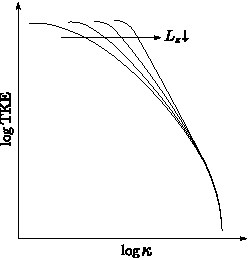
\includegraphics[width=0.4\textwidth]{chapter3/fig1}}
  \caption{Sketch of the TKE cascade distribution across the scales as the span is reduced.
By constricting the domain, the integral scale is reduced and the energy-containing scales can feed less energy to the inertial and dissipative scales.}
\label{fig:ek_sketch}
\end{figure}

These differences between 2-D and 3-D turbulence dynamics have a significant practical impact.
For example, the forces induced on a cylinder are larger in magnitude and variability in 2-D systems \citep{Mittal1995, Norberg2003}.
In an attempt to dissipate the energised vortical structures and to prevent the vortex-merging dynamics of 2-D turbulence, models based on the eddy-viscosity hypothesis (a.k.a. the Boussinesq hypothesis) are incorporated into 2-D strip-theory methods.
However, these models assume that the anisotropic Reynolds-stress tensor is proportional to the mean rate-of-strain tensor by the scalar eddy viscosity, a relation which has been proven inaccurate even for simple shear flows \citep[p. 94]{Pope2000} and can potentially yield incorrect forces induced to the cylinder.
A further complication for strip theory is that the presence of walls adds a production mechanism of 3-D turbulence which is able to generate very fine 3-D vortical structures even in highly anisotropic geometries.

A ``thick'' strip-theory method proposed by \cite{Bao2016} showed how strips with a certain thickness are able develop to 3-D turbulence when its span is larger than the wavelength of the Mode B instability of circular cylinders, $\lambda_z/D\approx1$ (see \aref{chapter:appendixA} for a summary of phenomena arising in flow past a circular cylinder at different Reynolds regimes).
In fact, this instability creates rib-like streamwise vortical structures along the main K\'{a}rm\'{a}n 2-D vortices \citep{Noack1999}.
Therefore, it can be argued that the two-dimensionalisation of the wake arises from the geometry constriction which prevents the rib-like vortices developing when there is not room enough for its natural wavelength.
However, the connection between wake and wall turbulence and the persistence of 3-D turbulent structures in constricted span flows has not been fully explored.

This work studies the geometry constriction effect on the turbulence nature of a flow past a circular cylinder at $Re=10^4$.
To do this, a series of simulations ranging from $L_z=10$ to pure 2-D planes have been considered.
As discussed above, the inclusion of a body boundary provides an important change to the turbulence production mechanisms compared to previous research as well as novel information on the transition and cross-over between 3-D and 2-D turbulence for very constricted domains in wall-generated turbulent shear flows.
Multiple turbulence statistics are presented for the wide range of constricted wakes, providing new data on the transition from 3-D to 2-D turbulence.

\section{Problem formulation}\label{sec:circular_cylinder_details}

This study considers flow past a circular cylinder with diameter $D$ aligned on the $z$ direction in a 3-D $\left(35\times20\times L_z\right)D$ rectangular domain, where $L_z$ is the non-dimensional span.
To study the span effect on the turbulence nature of the wake, the following cases have been considered: $L_z=10, \pi, 1, 0.5, 0.25, 0.1$ as well as a fully 2-D case.

\begin{figure}
	\vspace*{0.2cm}
  \centerline{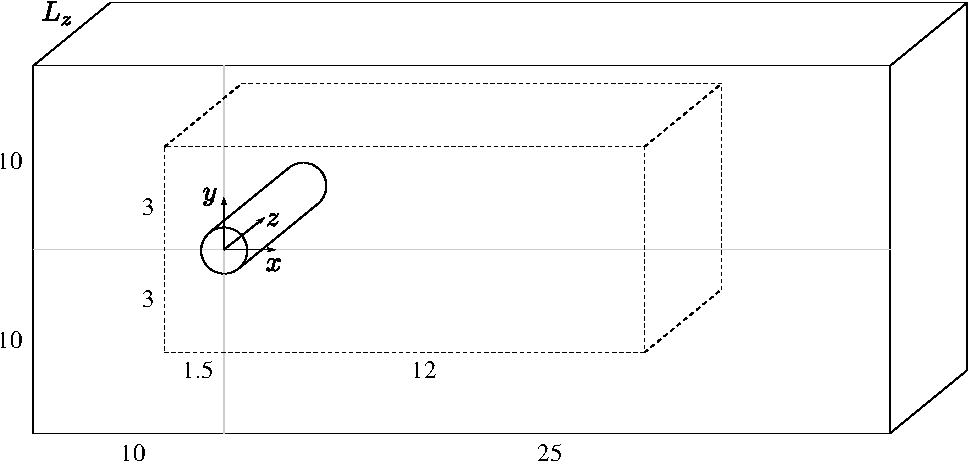
\includegraphics[width=0.8\textwidth]{chapter3/fig2}}
  \caption{Computational domain sketch non-dimensionalised with the cylinder diameter $D$.
  A very fine Cartesian grid domain (depicted in discontinuous lines) surrounds the cylinder and the close- and mid-wake regions.
  A stretched rectilinear grid (depicted in solid lines) transitions from the Cartesian grid to the boundaries.}
\label{fig:computational_domain}
\end{figure}

A Reynolds number of $Re=10^4$ is selected.
We define the Reynolds number as
\begin{equation}
Re=\frac{UD}{\nu},
\end{equation}
where $U$ is the scaling velocity and $\nu$ is the kinematic viscosity of the fluid.
Using this Reynolds number we ensure that the flow is well within the turbulence regime encompassing very different spatial and temporal scales in addition to the availability of DNS data \citep{Dong2005} which is used to validate our results in \aref{chapter:appendixB}.

The incompressible viscous fluid motion is described by the continuity equation and the non-dimensional Navier--Stokes momentum equations
\begin{eqnarray}
&\nabla\cdot\vect{u}=0,\label{eq:mass}\\
&\partial_{t}\vect{u}+\pars{\vect{u}\cdot\nabla} \vect{u}=-\nabla p+Re^{-1}\nabla^2\vect{u}.
\end{eqnarray}
Velocity and pressure fields are coupled with the pressure-Poisson equation. 
The initial condition is defined as $\vect{u}\left(\vect{x}, 0\right)=\left(1,0,0\right)$ in the fluid.
The boundary conditions are: a uniform velocity profile on the inlet boundary, a natural convection condition on the outlet boundary, a no-penetration slip condition on the upper and lower boundaries, a periodic condition on the spanwise direction boundaries and a no-slip velocity condition on the cylinder.
Periodic boundary conditions on the constricting planes are used as in previous studies on the cross-over of 2-D and 3-D turbulence for obstacle-free flows such as \cite{Smith1996}, \cite{Celani2010} and \cite{Biancofiore2014}.
This choice is made to avoid the artificial high intensity turbulence enhancements and the deterioration of the 2-D behaviour of the flow when a no-penetration condition is enforced on the constricting planes, as noted on \cite{Biancofiore2012} for obstacle-free turbulent wakes.
Other studies such as \cite{Bao2016} and \cite{Bao2019} also use a periodic spanwise condition for thick strips modelling long circular cylinders.

The numerical methods to solve the governing system of equations have been described in \cref{chapter:theoretical_background}. 
Particularly for the circular cylinder case, the domain is composed of a sufficiently fine Cartesian grid for the close- and mid-wake regions defined as $\left(L_x\times L_y\times L_z\right)D$, where $L_x$ and $L_y$ are the non-dimensional horizontal and vertical lengths respectively.
A stretched grid is considered for the regions far from the cylinder (see \fref{fig:computational_domain}).
A resolution of 90 cells per diameter in all spatial directions is chosen for the Cartesian grid subdomain.
The resolution in all spatial directions is kept constant as the span is reduced.

The 3-D simulations are started from a three-dimensionalised 2-D flow snapshot.
A time length of $t^*_0=200$ $(t^* = tU/D)$ is simulated before starting to record the flow statistics in order to achieve a statistically stationary state of the wake.
The flow statistics are then recorded for a total of $\Delta t^*=t^*-t^*_0=500$ convective time units (around 100 wake cycles).
A verification and validation of the wake turbulence dynamics of the investigated test case is included in \aref{chapter:appendixB}.
Finally, the turbulence statistics of the $L_z=10$ and $L_z=\pi$ cases are very similar as displayed in \fref{fig:TKE}a.
Hence, only the $L_z=\pi$ results are displayed on the other figures for clarity.

\section{Results and discussion}\label{Results and discussion}

The flow field is displayed in \fref{fig:instantaneous_vorticity} in terms of the instantaneous vorticity component $\omega_z$ as the span is varied.
The most striking feature is how the coherence of the K\'{a}rm\'{a}n vortices increases as the span is reduced.
However, even in highly-anisotropic geometries such as $L_z=0.25$, small-scale 3-D structures are generated from the cylinder wall.

An important result is that the two-dimensionalisation of these structures is faster (in the sense that it occurs closer to the cylinder) as the domain is constricted because of the geometry constriction and the natural rotation of the K\'{a}rm\'{a}n vortices.
The combination of these two mechanisms as a two-dimensionalisation method is also found in \cite{Smith1996} and \cite{Xia2011}.
For the $L_z\geq1$ cases, the 3-D small-scales structures detaching from the cylinder wall are not two-dimensionalised as rapidly.
In fact, it can be appreciated that only the far wake region of the $L_z=1$ case displays a coherent K\'{a}rm\'{a}n vortex.
This means that less anisotropic geometries promote a direct TKE cascade on the wake so that the 3-D dissipative structures are still sustained far from the cylinder.
\begin{figure}
	\vspace*{0.3cm}
  \centerline{\includegraphics[width=1\textwidth]{chapter3/fig3}}
  \caption{Instantaneous vorticity $\omega_z$ (red is positive, blue is negative) at the $z=L_z/2$ plane for: $(a)$ $L_z=0$, $(b)$ $L_z=0.1$, $(c)$ $L_z=0.25$, $(d)$ $L_z=0.5$, $(e)$ $L_z=1$, $(f)$ $L_z=\pi$.}
\label{fig:instantaneous_vorticity}
\end{figure}

Whether the wake turbulence dynamics is 2-D or 3-D is better captured on the TKE spectra which can be directly compared to classic turbulence theory.
For this, the Taylor's hypothesis is considered and the temporal spectrum at different points of the wake is calculated.
\fref{fig:velocity_spectras} a,b,c shows the temporal power spectrum (PS) of the $v$ velocity component at $(x,y)=(2,0.8),(4,0.8),(8,0.8)$.
The Welch method (using a time signal of 500 units split in 6 parts with 75\% overlapping) has been employed to compute the spectra at 8 different points along the span for each $(x,y)$ point.
These spectra are then averaged resulting in a single spectrum for each case.

First, note that all of the spectra display a peak around the $0.2$ non-dimensional frequency corresponding to the non-dimensional Strouhal number, $St=f_s D/U$, where $f_s$ is the vortex-shedding frequency.
A smaller harmonic peak around $0.4$ non-dimensional frequency is also found for the spectra at $(x,y)=(2,0.8),(4,0.8)$.
Second, the spectrum at the closest analysed point to the cylinder (\fref{fig:velocity_spectras}a) displays a 3-D turbulence behaviour with a $-5/3$ decaying rate with the exception of the pure 2-D and the $L_z=0.1$ cases.
For the latter cases, a decaying slope around $-11/3$ is found.
These 2-D flow spectra are steeper than the $-3$ rate predicted by the classical 2-D turbulence theory \citep{Kraichnan1967} because of the interaction of the coherent large-scale K\'{a}rm\'{a}n vortices, in agreement with the finds of \cite{Dritschel2008} and \cite{Biancofiore2014}.
The filamentary vorticity (filaments of vorticity around the coherent vortices) is likely to be destroyed by the interaction of the large-scale vortices rather than viscous effect (specially for high $Re$ flows), thus limiting its range of scales.
The coherent vortices induce a spiralling effect which limits the range of scales of incoherent filamentary vorticity \citep{Gilbert1988}.
On the other hand, as a $-5/3$ decay rate is captured for the $L_z=0.25$ case, it can be argued that 3-D turbulence is being generated from the cylinder wall even for highly reduced spans.

\begin{figure}
	\vspace*{0.3cm}
  \centerline{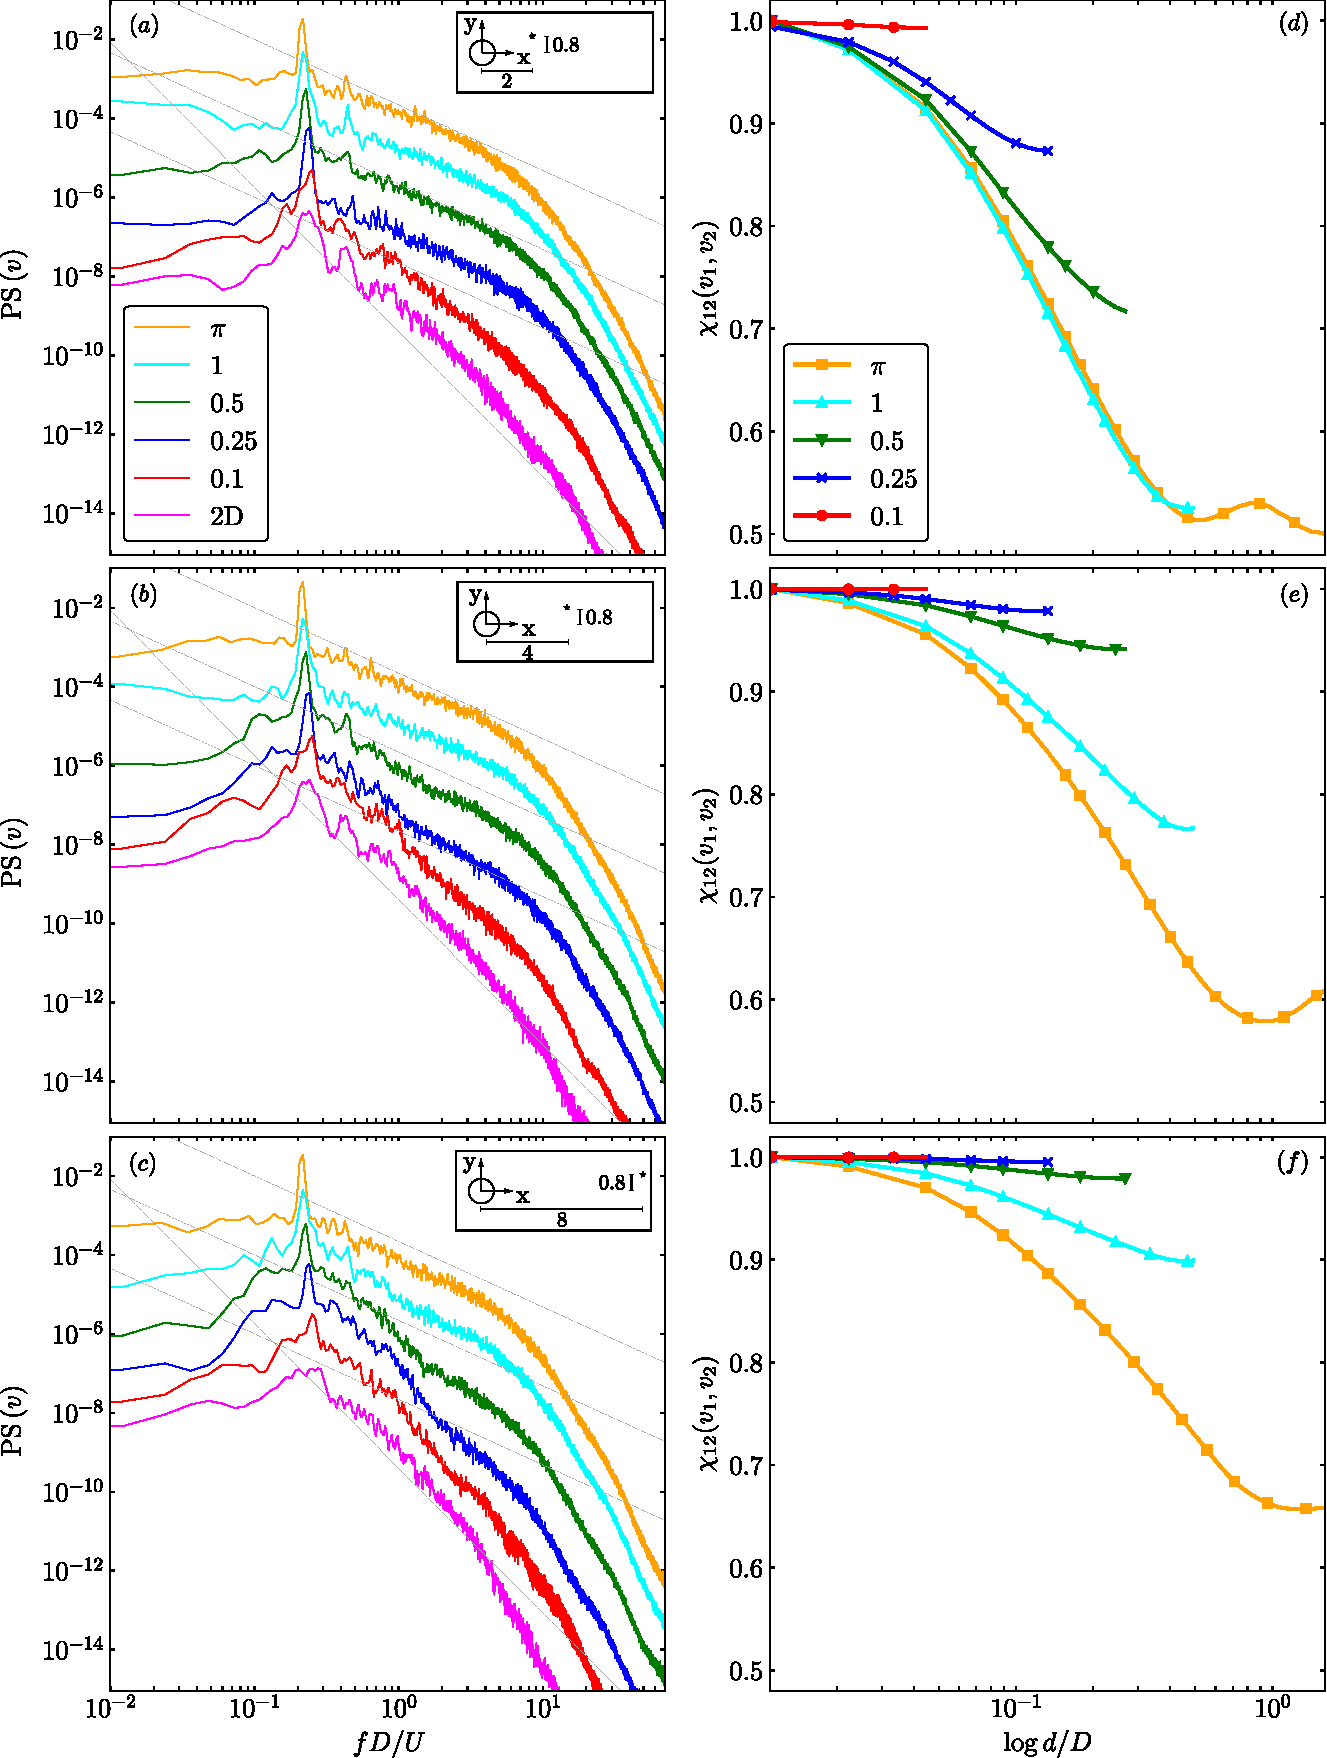
\includegraphics[width=1\textwidth]{chapter3/fig4}}
  \caption{Left: vertical velocity component temporal PS at different $\left(x,y\right)$ locations on the wake: $\left(a\right)=\left(2,0.8\right)$, $\left(b\right)=\left(4,0.8\right)$, $\left(c\right)=\left(8,0.8\right)$.
The PS lines of each case are shifted a factor of 10 for clarity and the vertical axis ticks correspond to the $L_z=\pi$ case.
The dashed lines have a $-11/3$ slope and the dotted lines have a $-5/3$ slope.
Right: two-point correlations along $z$ at the same $(x,y)$ locations as the left figures respectively.
The correlation value $\chi_{12}$ for a given $d$ corresponds to the averaged value of the multiple correlations of pairs of points separated a distance $d$ along the span.}
\label{fig:velocity_spectras}
\end{figure}

The $L_z=0.25$ and $L_z=0.5$ cases feature a decay rate that transitions from $-5/3$ to $-11/3$ as the spectra are computed further downstream from the cylinder.
In particular, both cases have $-5/3$ slopes in \fref{fig:velocity_spectras}a and $-11/3$ in \fref{fig:velocity_spectras}c, quantifying the turbulent two-dimensionalisation in the rotating wake.
Also note the coexistence of both 2-D and 3-D turbulence features for the $L_z=0.25,0.5$ and $L_z=1$ cases in \fref{fig:velocity_spectras}b and \fref{fig:velocity_spectras}c respectively.
The low-frequency structures behave mostly two-dimensionally (decay rate between $-3$ and $-11/3$, resulting from the presence of less coherent 2-D structures than the pure 2-D case) up to a certain point where a $-5/3$ rate is briefly recovered.
Hence, high-frequency structures interact in a 3-D fashion while low-frequency structures interact two-dimensionally.
This finding is in agreement with \cite{Smith1996} and \cite{Celani2010}.

Additionally, two-point correlations along the span have been analysed at the same $(x,y)$ locations as the PS plots (\fref{fig:velocity_spectras} d,e,f).
Given a distance $d$ along $z$ ranging from 0 to $L_z/2$, the two-point correlation is calculated with the temporal signals of the vertical velocity component at multiple pairs of points (namely $v_1$ and $v_2$) as follows
\begin{equation}
\chi_{12}\left(v_1(\vect{x},t), v_2(\vect{x}+\vect{r},t) \right) = \frac{\mathrm{cov}(v_1, v_2)}{\sqrt{\mathrm{cov}(v_1, v_1)\mathrm{cov}(v_2, v_2)}},
\end{equation}
where the distance vector is defined as $\vect{r}=(0,0,d)$.
The multiple correlation coefficients for a given $d$ are then averaged corresponding to a data point in the plots.

Very close to the cylinder (\fref{fig:velocity_spectras}d), the correlation coefficient quickly decreases with increasing $d$ for $L_z>0.1$.
This indicates the presence of 3-D structures near the body as also noted on the velocity spectrum plot counterpart.
Also, the decrease is more pronounced as the span increases.
For $L_z=\pi$, it is worth noting a local correlation coefficient maximum around $d \approx 0.9$.
This distance approximately corresponds to the Mode B instability wavelength $(\lambda_z)$.
Since the rib-like vortices associated with the Mode B instability (streamwise and crossflow vorticity) are not very well defined at this $Re$ regime \citep{Chyu1996}, the correlation increase is not as significant as at lower $Re$.
Still, $L_z=\pi$ is the only case displaying such phenomena because of the spanwise boundary conditions periodicity, which only allow the instability to develop if $L_z>\lambda_z$ (the $L_z=1$ case might be too critical to display such phenomenon considering also its intermittent nature).
The correlation coefficient increases when calculated further downstream as shown in \fref{fig:velocity_spectras}e and \ref{fig:velocity_spectras}f, evidencing again the wake two-dimensionalisation.

\begin{figure}
	\vspace*{0.3cm}
  \centerline{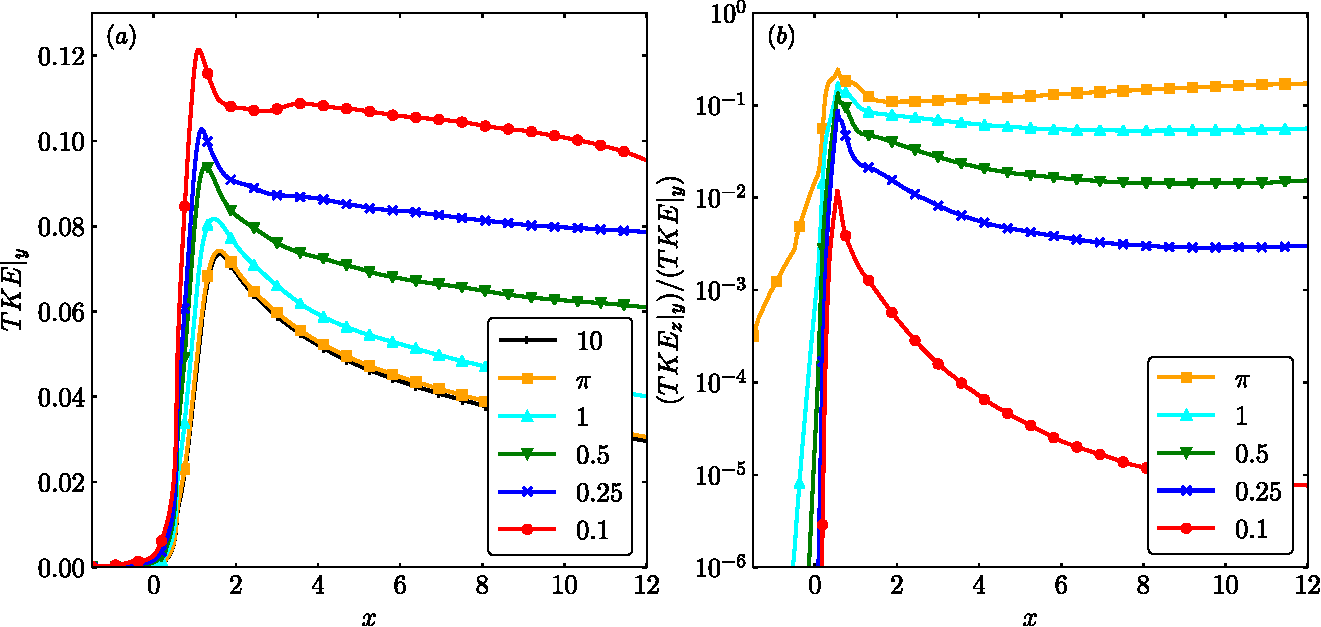
\includegraphics[width=1\textwidth]{chapter3/fig5}}
  \caption{TKE spatial plots.
The TKE is computed from the normal Reynolds stresses and averaged on the vertical direction: $(a)$ total TKE, $(b)$ ratio of the spanwise component $\overline{w'w'}$ to the total TKE.}
\label{fig:TKE}
\end{figure}

In summary, the transition to a 2-D wake is found at a certain point along the wake on all the cases with $L_z\le1$.
The combination of the large-scale rotation from the K\'{a}rm\'{a}n vortices plus the geometry constriction are mainly responsible for this phenomenon.
The main physical mechanism differing among the compared cases is the ability of the flow to develop Mode B-like 3-D structures in the wake as a result of a sufficiently long span.
The current $Re$ regime is characterised by a transition to turbulent flow at the shear layer (i.e. the TrSL2 regime) as reported in \cite{Bloor1964} and \cite{Kourta1987}.
We argue that when the span is too short for the Mode B instability to develop and thereby sustain these 3-D turbulent structures, the stratification effect of the K\'{a}rm\'{a}n vortices leads to the more coherent and energised wake seen in \fref{fig:velocity_spectras} d,e,f.

Next, the TKE along the $x$ direction, the Lumley triangle of turbulence and the ratio between the vortex-stretching and vortex-advecting terms are examined to further support the observed phenomena.
The TKE is defined as
\begin{equation}
TKE = \frac{1}{2}\left(\overline{u'u'}+\overline{v'v'}+\overline{w'w'}\right),
\end{equation}
where $\overline{\cdot}$ denotes a time average plus a spanwise average and the superscript $(\cdot)'$ denotes a fluctuating quantity such as $a'=a-\overline{a}$.
The six components of the Reynolds-stress tensor $\overline{u_i' u_j'}$ have been computed using the following relation
\begin{equation}
\overline{a'b'} = \overline{ab} - \overline{a}\overline{b}.
\end{equation}

\fref{fig:TKE} shows the streamwise spatial distribution of the TKE averaged along the $y$ direction from $-L_y/2$ to $L_y/2$ (noted as $\cdot|_y$).
From a general point of view, it can be observed that the total TKE (\fref{fig:TKE}a) peaks right after the recirculation region noting that the latter increases slightly with the span.
Also, the total TKE increases as the span is reduced because of the 2-D vortex-merging processes that generate larger and more energised vortical structures.
The contribution of the spanwise normal stress to the total TKE increases with the span as shown in \fref{fig:TKE}b.
Also, a decay of $\overline{w'w'}$ right after being generated from the cylinder wall can be noted and it becomes faster as the span is constricted.

The effect of the span on the TKE compared to the lift coefficient root mean square (r.m.s.) value $(\overline{C}_L)$ displays a quasi-linear relation as shown in \fref{fig:TKE_CL}.
Note that the drop on both values is more sensitive to the span constriction at the range where both 2-D and 3-D turbulence dynamics coexist, i.e. $0.25\le L_z\le1$.
On the other hand, a very small change of both values can be appreciated when 3-D turbulence fully dominates the wake, i.e. $L_z\ge\pi$.
Furthermore, as shown in \fref{fig:TKE}a, highly constricted domains yield large values of TKE because of the energised 2-D large-scale vortical structures present at the wake.
Even when small-scale 3-D structures are present in the close wake region and coexist with the large 2-D structures, the values of both the TKE and the $\overline{C}_L$ spike.

\begin{figure}
 \vspace*{0.3cm}
  \centerline{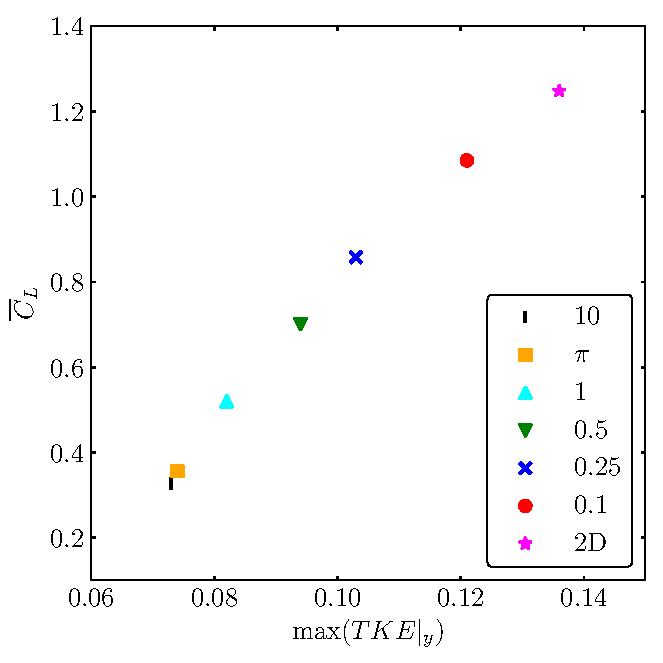
\includegraphics[width=0.5\textwidth]{chapter3/fig6}}
  \caption{Effect of the span constriction on the TKE and the $\overline{C}_L$.
The latter is calculated as $\overline{C}_L=|2F_y/(\rho U_\infty^2 D L_z)|_{\mathrm{rms}}$, where $F_y$ is the vertical lift force, $U_\infty$ is the free-stream velocity, and $\rho$ is the constant fluid density.}
\label{fig:TKE_CL}
\end{figure}

\begin{figure}
	\vspace*{0.3cm}
  \centerline{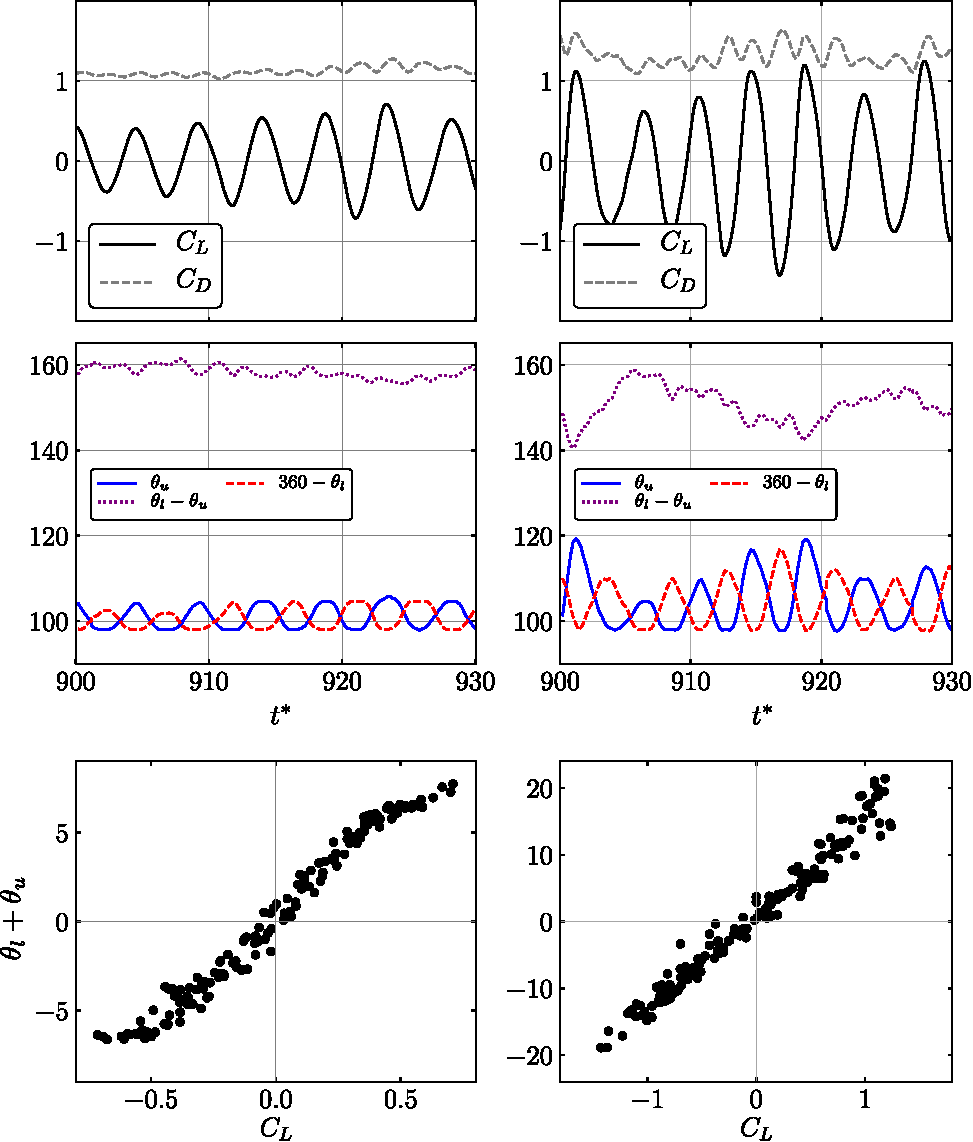
\includegraphics[width=0.9\textwidth]{chapter3/fig7}}
  \caption{Top: $C_L$ and $C_D$ temporal signals.
The latter is calculated as $C_D=2F_x/(\rho U_\infty^2 D L_z)$ and the former as detailed in \fref{fig:TKE_CL} (without the r.m.s norm).
Middle: upper $\theta_u$ and lower $\theta_l$ separation angles temporal signal.
The separation angle is calculated from the front stagnation point of the cylinder to the free shear layer separation point (vorticity practically 0 at the wall).
Bottom: correlation between the lift coefficient and the difference between $\theta_u$ and $360-\theta_l$.
Left: $L_z=\pi$.
Right: $L_z=0.5$.}
\label{fig:separation}
\end{figure}

In \fref{fig:separation}, the temporal signals of the lift and drag coefficients as well as the upper and lower separation angles of the free-shear layer are displayed for the $L_z=0.5$ and the $L_z=\pi$ cases.
The oscillation of the separation points increases as the span is constricted inducing larger forces on the cylinder.
A very high correlation of the upper and lower separation points angle with the lift coefficient is shown as well.
Again, the lack of the Mode B instability on the constricted cases yields more coherent 2-D vortical structures in the near wake region.
Therefore, the small-scale 3-D structures which normally dissipate most of the kinetic energy in 3-D turbulence are not present leading to high-intensity vortices.
This can be quantified by the enstrophy ($Z$) of the spanwise-averaged spanwise vorticity in the near wake region, $\Omega$ ($x \in [0.55, 2.1], y \in [-0.8, 0.8]$), which is time averaged for the same temporal length as the body forces signals as follows
\begin{equation}
Z = \int_\Omega\frac{1}{t_2-t_1}\int^{t_2}_{t_1}\frac{1}{L_z}\int^{L_z}_{0} \omega_z^{2} \,\,\mathrm{d}z\,\mathrm{d}t\,\mathrm{d}\Omega.
\label{eq:enstrophy}
\end{equation}
It can be observed in \tref{tab:enstrophy} that the enstrophy increases as the span is reduced, which can be understood as an increase of the rotational energy of the flow.

\begin{table}
  \begin{center}
\def~{\hphantom{0}}
  \begin{tabular}{lrrrrr}
  \toprule
       $L_z$ & $\pi$ & $1$  & $0.5$ & $0.25$ & $0.1$ \\
       \midrule
       $Z/Z_\pi$ & 1 & 1.32 & 1.71  & 2.07   & 2.47  \\
      \bottomrule
  \end{tabular}
  \caption{Near body enstrophy as defined in equation \ref{eq:enstrophy} for the different span cases.
$Z_\pi$ is the enstrophy of the $L_z=\pi$ case.}
  \label{tab:enstrophy}
  \end{center}
\end{table}

The highly energised coherent vortices forming at the near wake region for the constricted cases induce a larger convective force on the free-shear layer.
This translates to the large oscillations observed in \fref{fig:separation} and, ultimately, to the forces induced on the cylinder.
With this, it can be argued that the coherent 2-D structures have a greater impact on the forces induced to the cylinder than the 3-D small-scale structures when both are present.

\cite{Lumley1977} proposed the Lumley triangle of turbulence which provides a way to classify the anisotropic state of turbulence.
The anisotropy property of the Reynolds-stress tensor can be extracted with
\begin{equation}
b_{ij} = \frac{\overline{u_i' u_j'}}{\overline{u_k' u_k'}} - \frac{1}{3}\delta_{ij},
\end{equation}
where $\delta_{ij}$ is the Kronecker delta tensor and $b_{ij}$ is the anisotropic Reynolds-stress tensor (which evidently vanishes for isotropic turbulence).
This dimensionless and traceless tensor has two non-zero invariants, $II=-b_{ij}b_{ji}/2$ and $III=b_{ij}b_{jk}b_{ki}/3$.
These invariants are often rewritten as $\eta^2=-II/3$ and $\xi^3=III/2$ to better appreciate the nonlinear behaviour of the trajectories of return to isotropy of homogeneous turbulence \citep{Choi2001}.
It has been shown that all the possible turbulence states are mapped within the triangle \citep{Lumley1977, Lumley1979}.

The different states of turbulence are classified in the triangle as follows: the top right elbow indicates a one-dimensional (or one component) state with a single non-zero eigenvalue (the eigenvalues can be understood in physical terms as the normal stresses in the principal axes of the anisotropic Reynolds-stress tensor).
The top left elbow indicates a 2-D isotropic state where one eigenvalue vanishes and the two remaining are equal.
The top curve connecting the elbows indicates a 2-D turbulence state where one eigenvalue vanishes and the addition of the two remaining eigenvalues is constant.
The left and right straight lines correspond to a negative or positive $\left( \xi \right)$ axisymmetric state since one eigenvalue is smaller than the other two (which are equal) or greater than the other two (which are equal) respectively.
Finally, the $(0,0)$ point indicates 3-D isotropic turbulence since all of the anisotropic tensor eigenvalues vanish.

\begin{figure}
	\vspace*{0.3cm}
  \centerline{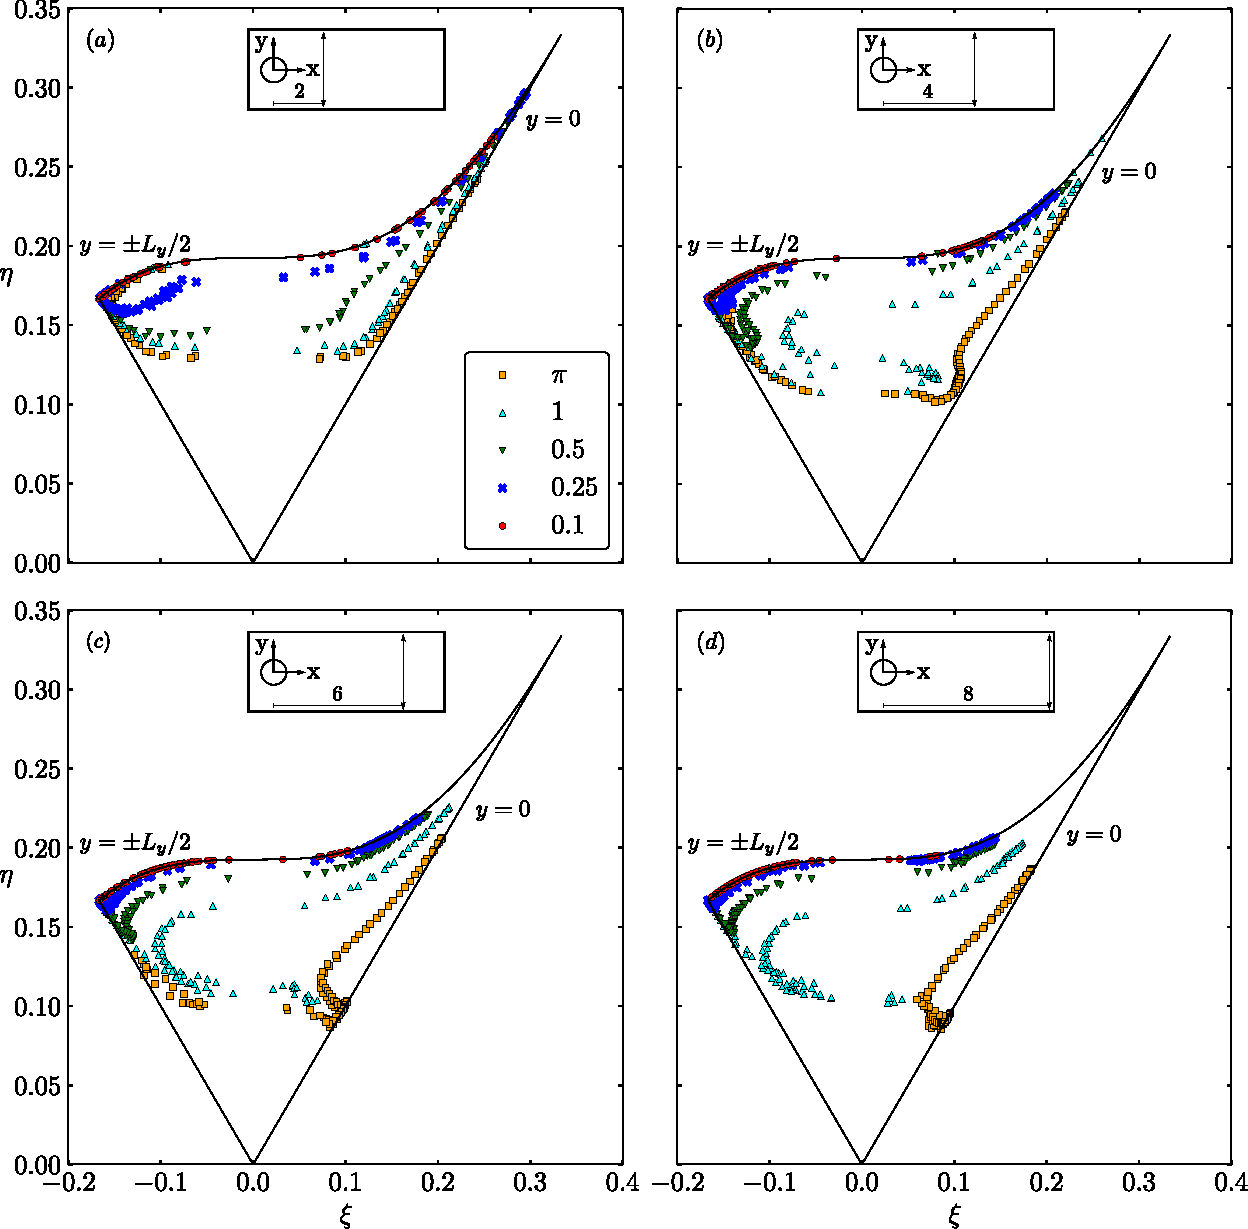
\includegraphics[width=1\textwidth]{chapter3/fig8}}
  \caption{Lumley triangle constructed across the wake width at: $(a)$ $x=2$, $(b)$ $x=4$, $(c)$ $x=6$, $(d)$ $x=8$.}
\label{fig:lumleys_triangle}
\end{figure}

\fref{fig:lumleys_triangle} displays the Lumley triangle constructed across the wake width at different $x$ locations.
Hence, every point in the triangle corresponds to a point in the domain and the collection of points for each case represents the collection of vertically aligned points in the domain at different $x$ locations on the wake.
It can be appreciated that all of the points are located within the triangle, therefore all of the computed Reynolds stresses are realisable (i.e. have positive and real eigenvalues).
In general, most of the cases transition from one state to another state of turbulence across the wake width.
Only for the almost 2-D case $\left(L_z=0.1\right)$, the state of turbulence is always 2-D (or two-component), since $\overline{w'w'}$ is effectively negligible everywhere.

As the triangle is constructed further downstream on the wake, the trajectories (or collection of points) of the $L_z=0.25$ and $L_z=0.5$ cases move closer to the 2-D turbulence state location (upper curve).
This emphasises once again the wake two-dimensionalisation caused by the large-scale vortical structures on cases with critical span which contain a cross-over of 2-D and 3-D turbulence, as shown in previous results.
In contrast, the $L_z=1$ and $L_z=\pi$ cases remain approximately at the same $\eta$ region showing that the two-dimensionalisation is not as effective.

Additionally, the trajectories present a negative axisymmetric almost two-component state for the locations far from the wake centreline, i.e. the location close to $y=\pm L_y/2$, since one of the normal turbulent stresses $(\overline{w'w'})$ is smaller than the others.
On the centreline, $\overline{v'v'}$ is larger than the other stresses causing a shift to the positive axisymmetric state.

A comparison of the different cases at the same $x$ location also shows a more noticeable 2-D turbulence state as the span is constricted.
This difference is less noticeable close to the cylinder (\fref{fig:lumleys_triangle}a), where even the $L_z=0.5$ case trajectory resembles the $L_z =\pi$ case.
Again, this evidences that 3-D turbulence is present close to the wall even in considerably constricted cases.

Consider now the vorticity transport equation (VTE) which can be written as
\begin{equation}
\partial_{t}\boldsymbol\omega+\pars{\vect{u}\cdot\nabla} \boldsymbol\omega=\pars{\boldsymbol\omega\cdot\nabla}\vect{u}+Re^{-1}\nabla^2\boldsymbol\omega,
\end{equation}
where $\boldsymbol\omega\left(\vect{x}, t\right) = \left(\omega_x, \omega_y, \omega_z\right)$ is the vorticity vector field defined as $\boldsymbol\omega=\nabla\times\vect{u}$.
The vortex-stretching term, $\pars{\boldsymbol\omega\cdot\nabla}\vect{u}$, is often pointed to as the term responsible for the direct energy cascade of the TKE.
The stretching of a vortex tube causes a reduction on its diameter while increasing the rotation speed of the vortex by conservation of angular momentum.
This term vanishes in the 2-D formulation of the VTE since the stretch of the vortex tube is perpendicular to the plane of rotation.
From this mathematical and physical difference, different turbulence dynamics is captured in 2-D or 3-D computations and, therefore, 3-D turbulence can be directly linked to this term.

\fref{fig:vortex_stretching} displays the modulus of the mean vortex-stretching term and its ratio $R$ to the mean vortex-advecting term.
These quantities are averaged in the vertical direction.
On \fref{fig:vortex_stretching}a, it can be observed that the vortex-stretching term decays faster while moving downstream from the cylinder for cases with shorter span.
The vortex-stretching decay demonstrates again the two-dimensionalisation of the flow by the large-scale vortices.
The ratio $R$ in \fref{fig:vortex_stretching}b shows that the vortex-advecting term decays faster (because of the wake momentum deficit) than the vortex-stretching term along the streamwise direction up to $x=6$ where the ratio is kept constant.
It can also be observed that the vortex-stretching term becomes as important as the vortex-advecting term with increasing span.
\begin{figure}
	\vspace*{0.3cm}
  \centerline{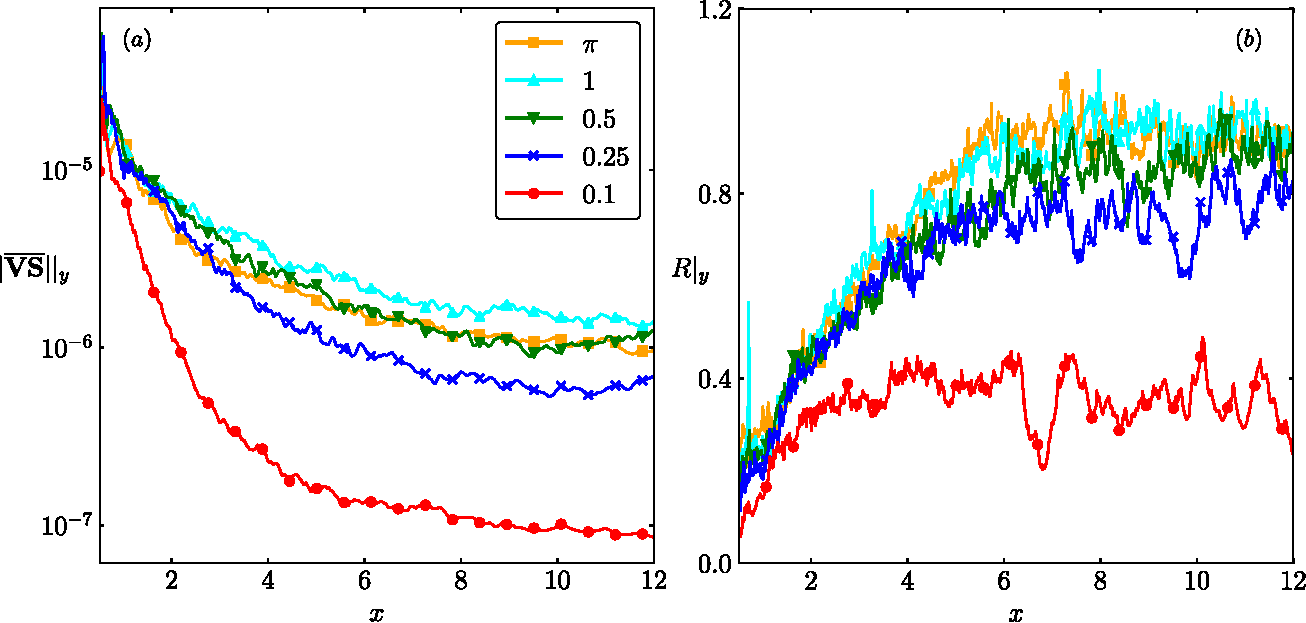
\includegraphics[width=1\textwidth]{chapter3/fig9}}
  \caption{$(a)$ Modulus of the mean vortex-stretching term averaged along the vertical direction.
$(b)$ Ratio of the modulus of the mean vortex-stretching term to the modulus of the mean vortex-advecting term averaged along the vertical direction.}
\label{fig:vortex_stretching}
\end{figure}

\section{Conclusion}\label{Conclusion}

The span effect on the turbulence dynamics of a flow past a circular cylinder at $Re=10^4$ has been investigated using spectra  and two-point correlations at different locations in the domain, the TKE along the wake, the separation points, the Lumley triangle of turbulence and the mean vortex-stretching term of the VTE.
It has been shown that 3-D turbulence is present even for highly constricted cases (for example $L_z=0.25$) which is generated by the cylinder wall (\fref{fig:velocity_spectras}a).
However, the small-scale structures rapidly get two-dimensionalised by the large-scale K\'{a}rm\'{a}n vortices when the span is 50\% of the diameter or less.
This is linked to the Mode B instability wavelength being longer than the periodic span, in agreement with \cite{Bao2016}.
Since the Mode B instability helps sustaining the turbulent structures advected from the shear layer, the lack of it prevents large-scale 3-D structures to be created and less dissipative structures can be sustained.
In this scenario, 2-D turbulence takes over and dominates the wake dynamics creating larger, stronger and more coherent vortices.
Ultimately, the coherent and energised vortical structures induce a larger convective force on the free-shear layer.
This translates to larger oscillations and, finally, higher forces on the cylinder.

The flow turbulence transition from 3-D to 2-D caused by a geometry constriction found in this work is in agreement with the physical mechanisms described in the obstacle-free turbulence work of \cite{Smith1996}, \cite{Celani2010} and \cite{Biancofiore2014}.
In the present study with solid boundaries, the main difference is found in the presence of small-scale 3-D turbulence even in highly constricted geometries $\left(L_z=0.25\right)$ which leads to a coexistence of 2-D and 3-D turbulence close to the cylinder wall.
This is observed not only in the $L_z=0.25$ case, but also for the $L_z=0.5$ and $L_z=1$ cases as shown in \fref{fig:velocity_spectras}b and \fref{fig:velocity_spectras}c respectively.
Note that the cross-over between 2-D and 3-D turbulence dynamics arises at different points in the spatial domain depending on the span length.
The shorter the span, the closer to the cylinder it takes place evidencing that the wake two-dimensionalisation transitions at different locations in function of the domain geometric anisotropy.

On the other hand, a very rapid two-dimensionalisation is found in the present cases because of the natural large-scale rotation motion of the K\'{a}rm\'{a}n vortices.
A large-scale rotation as a mechanism of two-dimensionalisation has been also found in other works such as \cite{Smith1996} and \cite{Xia2011}.
These two mechanisms combined yield to a rapid transition from the 3-D to 2-D turbulence dynamics when the span is shorter than the Mode B instability wavelength of the wake.
% ---------------------------------------------------------------- 
\end{document}
